%%%%%%%%%%%%%%%%%%%%%%%%%%%%%%%%%%%%%%%%%
% Beamer Presentation
% LaTeX Template
% Version 1.0 (10/11/12)
%
% This template has been downloaded from:
% http://www.LaTeXTemplates.com
%
% License:
% CC BY-NC-SA 3.0 (http://creativecommons.org/licenses/by-nc-sa/3.0/)
%
%%%%%%%%%%%%%%%%%%%%%%%%%%%%%%%%%%%%%%%%%

%----------------------------------------------------------------------------------------
%	PACKAGES AND THEMES
%----------------------------------------------------------------------------------------
\documentclass[aspectratio=169]{beamer}
\usepackage[portuges]{babel}
\usepackage[utf8]{inputenc}
\usepackage[alf]{abntex2cite}	
\usepackage[portuguese, linesnumbered, vlined, titlenumbered, ruled]{algorithm2e}
\usepackage{beamerthemesplit}
\usepackage{multirow}
\usepackage{scalefnt}
\usepackage{amssymb}
% \usepackage{tikz}
% \usetikzlibrary{matrix,backgrounds,matrix,positioning,arrows}
% \usetikzlibrary{patterns,arrows,decorations.pathreplacing}
% The Beamer class comes with a number of default slide themes
% which change the colors and layouts of slides. Below this is a list
% of all the themes, uncomment each in turn to see what they look like.

%\usetheme{default}
%\usetheme{AnnArbor}
%\usetheme{Antibes}
%\usetheme{Bergen}
%\usetheme{Berkeley}
%\usetheme{Berlin}
%\usetheme{Boadilla}
%\usetheme{CambridgeUS}
%\usetheme{Copenhagen}
%\usetheme{Darmstadt}
%\usetheme{Dresden}
%\usetheme{Frankfurt}
%\usetheme{Goettingen}
%\usetheme{Hannover}
%\usetheme{Ilmenau}
%\usetheme{JuanLesPins}
%\usetheme{Luebeck}
\usetheme{Madrid}
%\usetheme{Malmoe}
%\usetheme{Marburg}
%\usetheme{Montpellier}
%\usetheme{PaloAlto}
%\usetheme{Pittsburgh}
%\usetheme{Rochester}
%\usetheme{Singapore}
%\usetheme{Szeged}
%\usetheme{Warsaw}

% As well as themes, the Beamer class has a number of color themes
% for any slide theme. Uncomment each of these in turn to see how it
% changes the colors of your current slide theme.

%\usecolortheme{albatross}
%\usecolortheme{beaver}
%\usecolortheme{beetle}
%\usecolortheme{crane}
\usecolortheme{dolphin}
%\usecolortheme{dove}
%\usecolortheme{fly}
%\usecolortheme{lily}
%\usecolortheme{orchid}
%\usecolortheme{rose}
%\usecolortheme{seagull}
%\usecolortheme{seahorse}
%\usecolortheme{whale}
%\usecolortheme{wolverine}

%\setbeamertemplate{footline} % To remove the footer line in all slides uncomment this line
%\setbeamertemplate{footline}[page number] % To replace the footer line in all slides with a simple slide count uncomment this line

%\setbeamertemplate{navigation symbols}{} % To remove the navigation symbols from the bottom of all slides uncomment this line


\usepackage{graphicx} % Allows including images
\usepackage{booktabs} % Allows the use of \toprule, \midrule and \bottomrule in tables

%----------------------------------------------------------------------------------------
%	TITLE PAGE
%----------------------------------------------------------------------------------------
\title[Grafos]{Algoritmos e Estrutura de Dados}
\subtitle{Grafos}
\author[Frederico Santos de Oliveira]{prof. Frederico Santos de Oliveira}
\institute[UFMT]{Universidade Federal de Mato Grosso\\ Faculdade de Engenharia}
\date{}


\begin{document}

%------------------------------------------------
\begin{frame}
\titlepage % Print the title page as the first slide

\begin{figure}[!h]
  \centering
  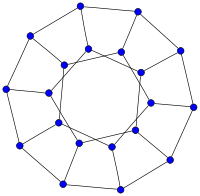
\includegraphics[width=70pt]{imagens/introducao.png}
  \label{fig_introducao}
\end{figure}
\end{frame}

%------------------------------------------------

\begin{frame}
\frametitle{Roteiro} % Table of contents slide, comment this block out to remove it
\tableofcontents % Throughout your presentation, if you choose to use \section{} and \subsection{} commands, these will automatically be printed on this slide as an overview of your presentation
\end{frame}

%----------------------------------------------------------------------------------------
%	PRESENTATION SLIDES
%----------------------------------------------------------------------------------------

%%%%%%%%%%%%%%%%%%%%%%%%%%%%%%%%%%%%%%%%%%%%%%%%%%%%%%%%%%%%%%%%%%%%%%%%%%%%%%%%%%%%%%%%%%%%%%%%%%%%%%%%%%%%%%%%%%%%%%%%%%%%%%
\section{Objetivos}
%%%%%%%%%%%%%%%%%%%%%%%%%%%%%%%%%%%%%%%%%%%%%%%%%%%%%%%%%%%%%%%%%%%%%%%%%%%%%%%%%%%%%%%%%%%%%%%%%%%%%%%%%%%%%%%%%%%%%%%%%%%%%%

\begin{frame}
\frametitle{Objetivos}

Esta aula tem como objetivos:

\begin{enumerate}
\item Formalizar a definição de grafo,
\item Introduzir os conceitos de isomorfismo, caminho, circuito, subgrafo, conexão, componente e grafo aleatório. 
\end{enumerate}
\end{frame}

%%%%%%%%%%%%%%%%%%%%%%%%%%%%%%%%%%%%%%%%%%%%%%%%%%%%%%%%%%%%%%%%%%%%%%%%%%%%%%%%%%%%%%%%%%%%%%%%%%%%%%%%%%%%%%%%%%%%%%%%%%%%%%
\section{Motivação} % Sections can be created in order to organize your presentation into discrete blocks, all sections and subsections are automatically printed in the table of contents as an overview of the talk
%%%%%%%%%%%%%%%%%%%%%%%%%%%%%%%%%%%%%%%%%%%%%%%%%%%%%%%%%%%%%%%%%%%%%%%%%%%%%%%%%%%%%%%%%%%%%%%%%%%%%%%%%%%%%%%%%%%%%%%%%%%%%%

\begin{frame}
\frametitle{Motivação}
\begin{itemize}
\item Muitas aplicações em computação necessitam considerar um conjunto de conexões entre pares de objetos:
\begin{itemize}
\item Existe um caminho para ir de um objeto a outro seguindo as conexões?
\item Qual é a menor distância entre dois objetos?
\item Quantos outros objetos podem ser alcançados a partir de um determinado objeto?
\end{itemize}
\item Existe um tipo abstrato chamado {\bf grafo} que é usado para modelar tais situações.
\end{itemize}
\end{frame}

%%%%%%%%%%%%%%%%%%%%%%%%%%%%%%%%%%%%%%%%%%%%%%%%%%%%%%%%%%%%%%%%%%%%%%%%%%%%%%%%%%%%%%%%%%%%%%%%%%%%%%%%%%%%%%%%%%%%%%%%%%%%%%

\begin{frame}
\frametitle{Aplicações}
\begin{itemize}
\item Alguns exemplos de problemas práticos que podem ser resolvidos através de uma modelagem em grafos:
\begin{itemize}
\item Ajudar máquinas de busca a localizar informação relevante na Web.
\item Descobrir as melhores combinações entre vagas de emprego e pessoas com enviaram currículo.
\item Descobrir qual é o roteiro mais curto para visitar as principais cidades de uma região turística.
\end{itemize}
\end{itemize}
\end{frame}

%%%%%%%%%%%%%%%%%%%%%%%%%%%%%%%%%%%%%%%%%%%%%%%%%%%%%%%%%%%%%%%%%%%%%%%%%%%%%%%%%%%%%%%%%%%%%%%%%%%%%%%%%%%%%%%%%%%%%%%%%%%%%%
\section{Introdução} % Sections can be created in order to organize your presentation into discrete blocks, all sections and subsections are automatically printed in the table of contents as an overview of the talk
%%%%%%%%%%%%%%%%%%%%%%%%%%%%%%%%%%%%%%%%%%%%%%%%%%%%%%%%%%%%%%%%%%%%%%%%%%%%%%%%%%%%%%%%%%%%%%%%%%%%%%%%%%%%%%%%%%%%%%%%%%%%%%

\begin{frame}
\frametitle{Introdução}
\begin{itemize}
\item Um grafo é um par(V,A) em que V é um conjunto de vértices e A é o conjunto de arestas.  
\end{itemize}
\begin{figure}[!h]
  \centering
  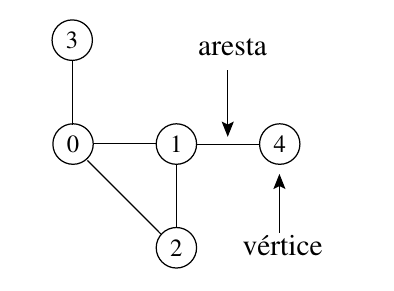
\includegraphics[width=150pt]{imagens/exemplo_grafo.png}
  \label{fig_exemplo_grafo1}
\end{figure}
\end{frame}

%%%%%%%%%%%%%%%%%%%%%%%%%%%%%%%%%%%%%%%%%%%%%%%%%%%%%%%%%%%%%%%%%%%%%%%%%%%%%%%%%%%%%%%%%%%%%%%%%%%%%%%%%%%%%%%%%%%%%%%%%%%%%%

\begin{frame}
\frametitle{Introdução}
\begin{itemize}
\item Uma aresta $(a,b)$ será denotada simplesmente por $ab$ ou por $ba$.  
\item Dizemos que a aresta $ab$ incide em $a$ e em $b$, e que $a$ e $b$ são as pontas da aresta. 
\item Se $ab$ é uma aresta, dizemos que os vértices $a$ e $b$ são vizinhos ou adjacentes.
\end{itemize}
\end{frame}

%%%%%%%%%%%%%%%%%%%%%%%%%%%%%%%%%%%%%%%%%%%%%%%%%%%%%%%%%%%%%%%%%%%%%%%%%%%%%%%%%%%%%%%%%%%%%%%%%%%%%%%%%%%%%%%%%%%%%%%%%%%%%%
\subsection{Definições}
%%%%%%%%%%%%%%%%%%%%%%%%%%%%%%%%%%%%%%%%%%%%%%%%%%%%%%%%%%%%%%%%%%%%%%%%%%%%%%%%%%%%%%%%%%%%%%%%%%%%%%%%%%%%%%%%%%%%%%%%%%%%%%

\begin{frame}{Definições}{Grafos Direcionados}
\begin{itemize}
\item Um grafo {\bf direcionado} $G$ é um par $(V, A)$, onde $V$ é um conjunto finito de vértices e $A$ é uma relação binária em $V$.
\begin{itemize}
\item Uma aresta $(a, b)$ sai do vértice $a$ e entra no vértice $b$. O vértice $a$ é adjacente ao vértice $b$.
\item Podem existir arestas de um vértice para ele mesmo, chamadas de self-loops.
\end{itemize}
\end{itemize}
\begin{figure}[!h]
  \centering
  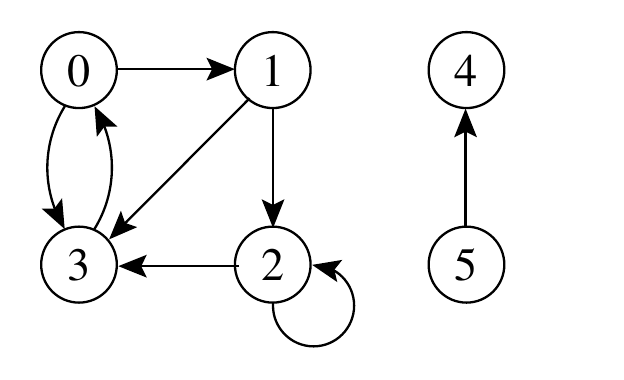
\includegraphics[width=150pt]{imagens/exemplo_grafo_direcionado.png}
  \label{fig_exemplo_grafo_direcionado}
\end{figure}
\end{frame}

%%%%%%%%%%%%%%%%%%%%%%%%%%%%%%%%%%%%%%%%%%%%%%%%%%%%%%%%%%%%%%%%%%%%%%%%%%%%%%%%%%%%%%%%%%%%%%%%%%%%%%%%%%%%%%%%%%%%%%%%%%%%%%

\begin{frame}{Definições}{Grafos não-direcionados}
\begin{itemize}
\item  Um grafo {\bf não-direcionado} $G$ é um par $(V, A)$, onde o conjunto de arestas $A$ é constituído de pares de vértices não ordenados.
\begin{itemize}
\item As arestas $(a, b)$ e $(b, a)$ são consideradas como uma única aresta.
\item A relação de adjacência é simétrica.
\item Self-loops não são permitidos.
\end{itemize}
\end{itemize}
\begin{figure}[!h]
  \centering
  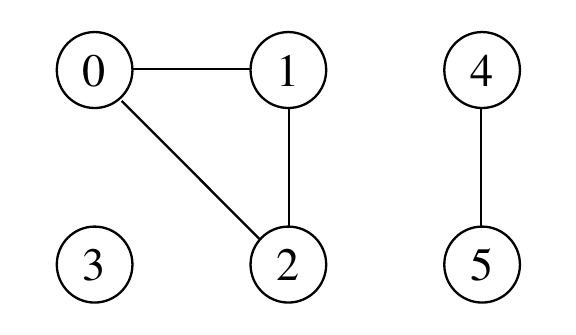
\includegraphics[width=150pt]{imagens/exemplo_grafo_nao_direcionado.png}
  \label{fig_exemplo_grafo_nao_direcionado}
\end{figure}
\end{frame}

%%%%%%%%%%%%%%%%%%%%%%%%%%%%%%%%%%%%%%%%%%%%%%%%%%%%%%%%%%%%%%%%%%%%%%%%%%%%%%%%%%%%%%%%%%%%%%%%%%%%%%%%%%%%%%%%%%%%%%%%%%%%%%

\begin{frame}{Definições}{Grau de um Vértice}
Em grafos não-direcionados:
\begin{itemize}
\item O {\bf grau} de um vértice é o número de arestas que incidem nele.
\item Um vértice de grau zero é chamado de vértice isolado ou não-conectado.
\item Ex.: O vértice 1 tem grau 2 e o vértice 3 é isolado.
\end{itemize}

\begin{figure}[!h]
  \centering
  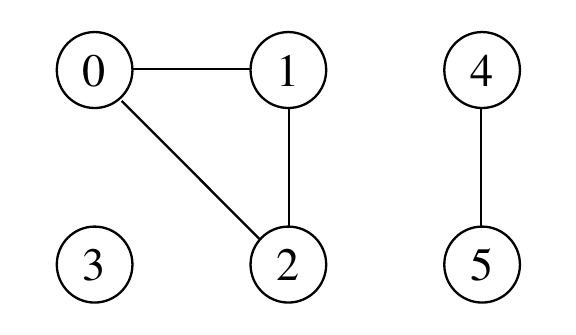
\includegraphics[width=100pt]{imagens/exemplo_grafo_nao_direcionado.png}
  \label{fig_exemplo_grau_grafo_nao_direcionado}
\end{figure}

\end{frame}

%%%%%%%%%%%%%%%%%%%%%%%%%%%%%%%%%%%%%%%%%%%%%%%%%%%%%%%%%%%%%%%%%%%%%%%%%%%%%%%%%%%%%%%%%%%%%%%%%%%%%%%%%%%%%%%%%%%%%%%%%%%%%%

\begin{frame}{Definições}{Grau de um Vértice}
Em grafos direcionados
\begin{itemize} 
\item O {\bf grau} de um vértice é o número de arestas que saem dele (grau de saída) mais o número de arestas que chegam nele (grau de entrada).
\item Ex.: O vértice 2 tem grau de entrada 2 e grau de saída 2, portanto possui grau 4.
\end{itemize}
\begin{figure}[!h]
  \centering
  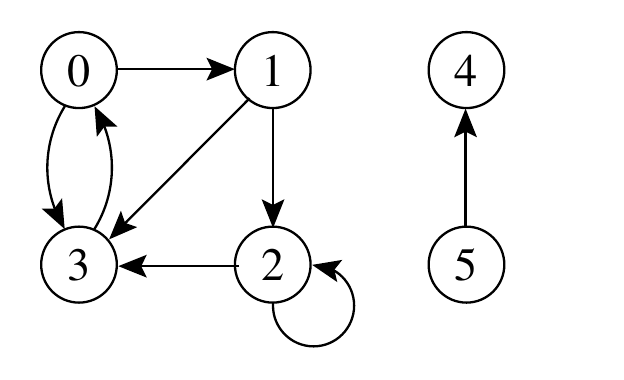
\includegraphics[width=100pt]{imagens/exemplo_grafo_direcionado.png}
  \label{fig_exemplo_grau_grafo_direcionado}
\end{figure}
\end{frame}

%%%%%%%%%%%%%%%%%%%%%%%%%%%%%%%%%%%%%%%%%%%%%%%%%%%%%%%%%%%%%%%%%%%%%%%%%%%%%%%%%%%%%%%%%%%%%%%%%%%%%%%%%%%%%%%%%%%%%%%%%%%%%%

\begin{frame}{Definições}{Caminho entre Vértices}
\begin{itemize}
\item Um {\bf caminho} de comprimento $k$ de um vértice $x$ a um vértice $y$ em um grafo $G = (V, A)$ é uma sequência de vértices $(v_0 , v_1 , v_2 , ... , v_k)$ tal que $x = v_0$ e $y = v_k$ , e $(v_{i-1}, v_i ) \in A$ para $i = 1, 2, ... , k$.
\item O comprimento de um caminho é o número de arestas nele, isto é, o caminho contém os vértices $v_0 , v_1 , v_2 , ... , v_k$ e as arestas $(v_0 , v_1)$, $(v_1 , v_2), ... , (v_{k-1} , v_k)$.
\item Se existir um caminho $c$ de $x$ a $y$ então $y$ é alcançável a partir de $x$ via $c$.
\item Um caminho é simples se todos os vértices do caminho são distintos.
\item Ex.: O caminho $(0, 1, 2, 3)$ é simples e tem comprimento $3$. O caminho $(1, 3, 0, 3)$ não é simples.
\end{itemize}
\begin{figure}[!h]
  \centering
  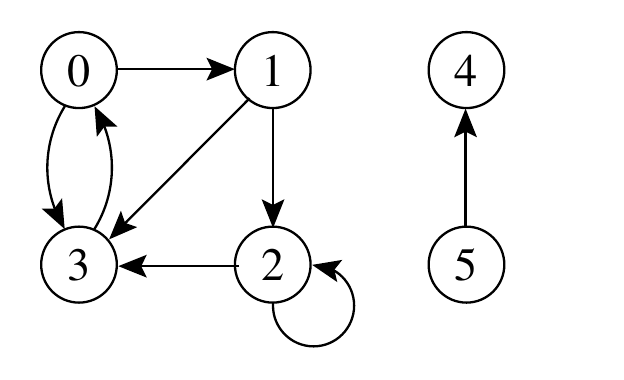
\includegraphics[width=100pt]{imagens/exemplo_grafo_direcionado.png}
  \label{fig_exemplo_caminho}
\end{figure}
\end{frame}

%%%%%%%%%%%%%%%%%%%%%%%%%%%%%%%%%%%%%%%%%%%%%%%%%%%%%%%%%%%%%%%%%%%%%%%%%%%%%%%%%%%%%%%%%%%%%%%%%%%%%%%%%%%%%%%%%%%%%%%%%%%%%%

\begin{frame}{Definições}{Ciclos}
Em um grafo direcionado:
\begin{itemize}
\item Um caminho $(v_0 , v_1 , ... , v_k )$ forma um {\bf ciclo} se $v_0 = v_k$ e o caminho contém pelo menos uma aresta.
\item O ciclo é simples se os vértices $v_1, v_2 , ... , v_k$ são distintos.
\item O self-loop é um ciclo de tamanho 1.
\item Dois caminhos $(v_0 , v_1 , ... , v_k )$ e $(v_0', v_1' , ... , v_k')$ formam o mesmo ciclo se existir um inteiro $j$ tal que $v_{i}' = v_{(i+j) \mod k} \textrm{ para } i = 0, 1, ... , k - 1$.
\item Ex.: O caminho $(0, 1, 2, 3, 0)$ forma um ciclo.
\item O caminho $(0, 1, 3, 0)$ forma o mesmo ciclo que os caminhos $(1, 3, 0, 1)$ e $(3, 0, 1, 3)$.
\end{itemize}
\begin{figure}[!h]
  \centering
  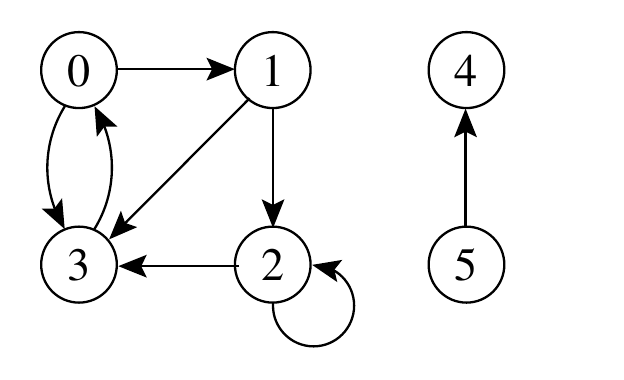
\includegraphics[width=150pt]{imagens/exemplo_grafo_direcionado.png}
  \label{fig_exemplo_ciclo}
\end{figure}
\end{frame}

%%%%%%%%%%%%%%%%%%%%%%%%%%%%%%%%%%%%%%%%%%%%%%%%%%%%%%%%%%%%%%%%%%%%%%%%%%%%%%%%%%%%%%%%%%%%%%%%%%%%%%%%%%%%%%%%%%%%%%%%%%%%%%

\begin{frame}{Definições}{Ciclos}
Em um grafo não-direcionado:
\begin{itemize}
\item Um caminho $(v_0 , v_1 , ... , v_k )$ forma um {\bf ciclo} se $v_0 = v_k$ e o caminho contém pelo menos três arestas.
\item O ciclo é simples se os vértices $v_1 , v_2 , ..., v_k$ são distintos.
\item Ex.: O caminho $(0, 1, 2, 0)$ é um ciclo.
\end{itemize}
\begin{figure}[!h]
  \centering
  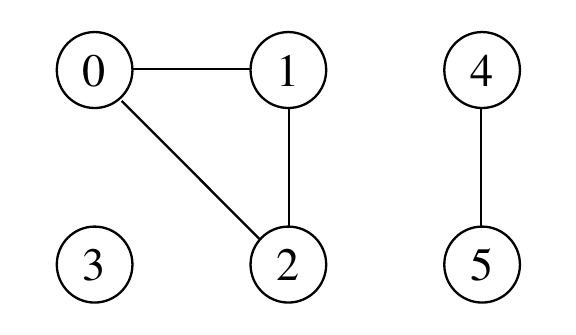
\includegraphics[width=150pt]{imagens/exemplo_grafo_nao_direcionado.png}
  \label{fig_exemplo_ciclo_grafo_nao_direcionado}
\end{figure}
\end{frame}

%%%%%%%%%%%%%%%%%%%%%%%%%%%%%%%%%%%%%%%%%%%%%%%%%%%%%%%%%%%%%%%%%%%%%%%%%%%%%%%%%%%%%%%%%%%%%%%%%%%%%%%%%%%%%%%%%%%%%%%%%%%%%%

\begin{frame}{Definições}{Componentes Conectados}
\begin{itemize}
\item Um grafo não-direcionado é {\bf conectado} se cada par de vértices está conectado por um caminho.
\item Os componentes conectados são as porções conectadas de um grafo.
\item Um grafo não-direcionado é conectado se ele tem exatamente um componente conectado.
\item Ex.: Os componentes são: $\{0, 1, 2\}, \{4, 5\}$ e  ${3}$.
\end{itemize}
\begin{figure}[!h]
  \centering
  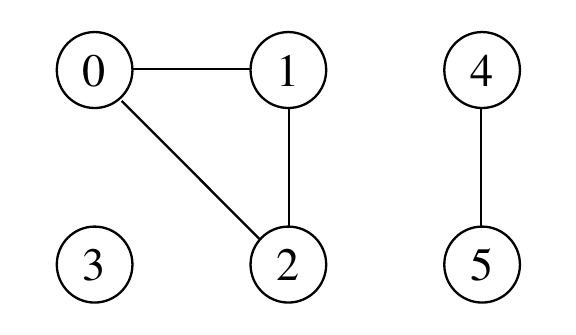
\includegraphics[width=150pt]{imagens/exemplo_grafo_nao_direcionado.png}
  \label{fig_exemplo_componente_conectado}
\end{figure}
\end{frame}
 
%%%%%%%%%%%%%%%%%%%%%%%%%%%%%%%%%%%%%%%%%%%%%%%%%%%%%%%%%%%%%%%%%%%%%%%%%%%%%%%%%%%%%%%%%%%%%%%%%%%%%%%%%%%%%%%%%%%%%%%%%%%%%%

\begin{frame}{Definições}{Componentes Fortemente Conectados}
\begin{itemize}
\item Um grafo direcionado $G = (V, A)$ é {\bf fortemente conectado} se dois vértices quaisquer são alcançáveis um a partir do outro.
\item Os componentes fortemente conectados de um grafo direcionado são conjuntos de vértices sob a relação ``são mutuamente alcançáveis''.
\item Um grafo direcionado fortemente conectado tem apenas um componente fortemente conectado.
\item Ex.: $\{0, 1, 2, 3\}$, $\{4\}$ e $\{5\}$ são os componentes fortemente conectados, $\{4, 5\}$ não o é, pois o vértice 5 não é alcançável a partir do vértice 4.

\end{itemize}
\begin{figure}[!h]
  \centering
  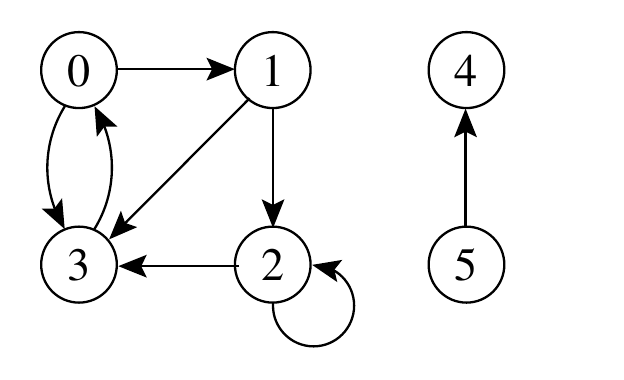
\includegraphics[width=150pt]{imagens/exemplo_grafo_direcionado.png}
  \label{fig_exemplo_componente_fortemente_conectado}
\end{figure}
\end{frame}

%%%%%%%%%%%%%%%%%%%%%%%%%%%%%%%%%%%%%%%%%%%%%%%%%%%%%%%%%%%%%%%%%%%%%%%%%%%%%%%%%%%%%%%%%%%%%%%%%%%%%%%%%%%%%%%%%%%%%%%%%%%%%% 

\begin{frame}{Definições}{Isomorfismo}
\begin{itemize}
\item $G = (V, A)$ e $G' = (V' , A')$ são {\bf isomorfos} se existir uma bijeção $f : V \rightarrow V'$ tal que $(u, v) \in A$ se e somente se $(f (u), f (v)) \in A'$.
\item Em outras palavras, é possível re-rotular os vértices de $G$ para serem rótulos de $G'$ mantendo as arestas correspondentes em $G$ e $G'$.
\end{itemize}
\begin{figure}[!h]
  \centering
  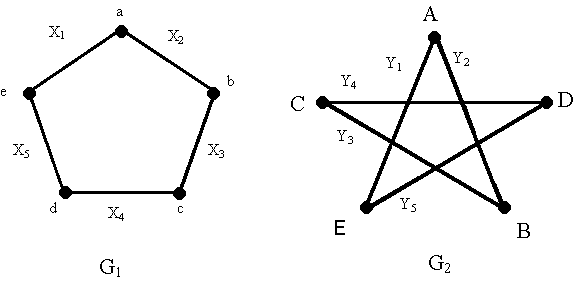
\includegraphics[width=250pt]{imagens/exemplo_isomorfismo1.png}
  \label{fig_exemplo_isomorfismo1}
\end{figure}
\end{frame}

%%%%%%%%%%%%%%%%%%%%%%%%%%%%%%%%%%%%%%%%%%%%%%%%%%%%%%%%%%%%%%%%%%%%%%%%%%%%%%%%%%%%%%%%%%%%%%%%%%%%%%%%%%%%%%%%%%%%%%%%%%%%%% 

\begin{frame}{Definições}{Isomorfismo}
\begin{figure}[!h]
  \centering
  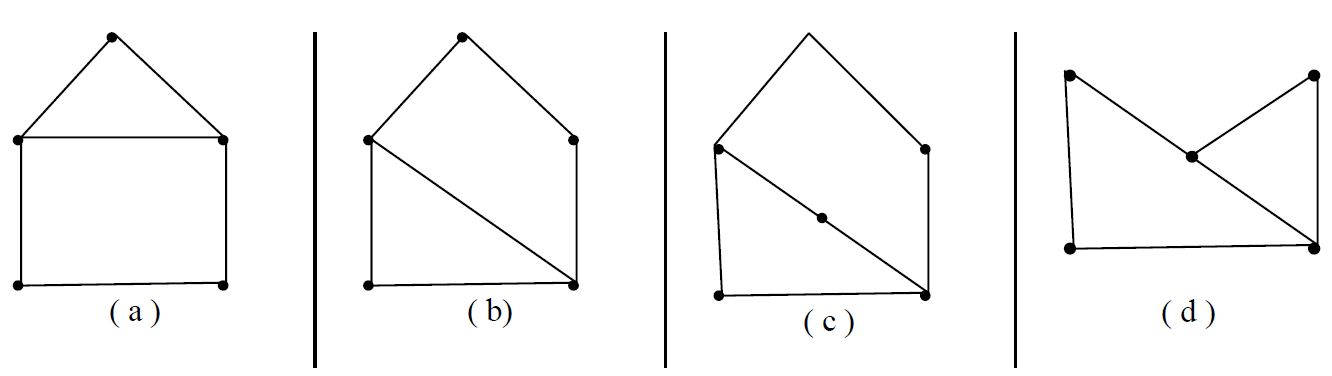
\includegraphics[width=250pt]{imagens/exemplo_isomorfismo2.jpg}
  \label{fig_exemplo_isomorfismo2}
\end{figure}
\end{frame}

%%%%%%%%%%%%%%%%%%%%%%%%%%%%%%%%%%%%%%%%%%%%%%%%%%%%%%%%%%%%%%%%%%%%%%%%%%%%%%%%%%%%%%%%%%%%%%%%%%%%%%%%%%%%%%%%%%%%%%%%%%%%%% 

\begin{frame}{Definições}{Isomorfismo}
\begin{figure}[!h]
  \centering
  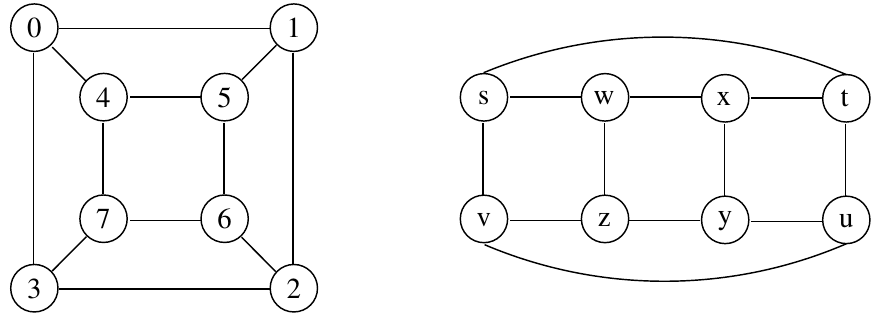
\includegraphics[width=250pt]{imagens/exemplo_isomorfismo3.png}
  \label{fig_exemplo_isomorfismo3}
\end{figure}
\end{frame}

%%%%%%%%%%%%%%%%%%%%%%%%%%%%%%%%%%%%%%%%%%%%%%%%%%%%%%%%%%%%%%%%%%%%%%%%%%%%%%%%%%%%%%%%%%%%%%%%%%%%%%%%%%%%%%%%%%%%%%%%%%%%%% 

\begin{frame}{Definições}{Subgrafos}
\begin{itemize}
\item Um grafo $G' = (V' , A')$ é um {\bf subgrafo} de $G = (V, A)$ se $V' \subseteq V$ e $A' \subseteq A$.
\item Dado um conjunto $V' \subseteq V$ , o subgrafo induzido por $V'$ é o grafo $G' = (V' , A' )$, onde $A' = \{(u, v) \in A|u, v \in V' \}$.
\item Ex.: Subgrafo induzido pelo conjunto de vértices $\{1, 2, 4, 5\}$.
\end{itemize}
\begin{figure}[!h]
  \centering
  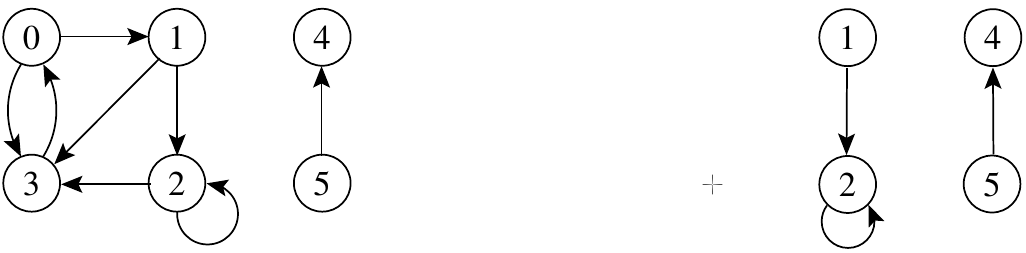
\includegraphics[width=300pt]{imagens/exemplo_subgrafo.png}
  \label{fig_exemplo_subgrafo}
\end{figure}
\end{frame}

%%%%%%%%%%%%%%%%%%%%%%%%%%%%%%%%%%%%%%%%%%%%%%%%%%%%%%%%%%%%%%%%%%%%%%%%%%%%%%%%%%%%%%%%%%%%%%%%%%%%%%%%%%%%%%%%%%%%%%%%%%%%%% 

\begin{frame}{Definições}{Versão Direcionada de um Grafo Não-Direcionado}
\begin{itemize}
\item A {\bf versão direcionada de um grafo não-direcionado} $G = (V, A)$ é um grafo direcionado $G' = (V' , A')$ onde $(u, v) \in A'$ se e somente se
$(u, v) \in A$.
\item Cada aresta não-direcionada $(u, v)$ em $G$ é substituída por duas arestas direcionadas $(u, v)$ e $(v, u)$.
\item Em um grafo direcionado, um vizinho de um vértice $u$ é qualquer vértice adjacente a $u$ na versão não-direcionada de $G$.
\end{itemize}
\begin{figure}[!h]
  \centering
  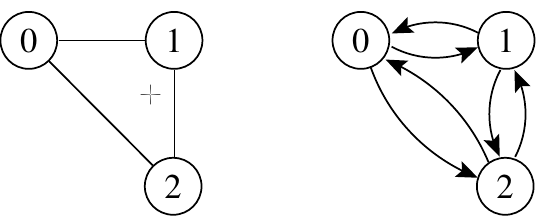
\includegraphics[width=200pt]{imagens/exemplo_versao_direcionada.png}
  \label{fig_exemplo_versao_direcionada}
\end{figure}
\end{frame}

%%%%%%%%%%%%%%%%%%%%%%%%%%%%%%%%%%%%%%%%%%%%%%%%%%%%%%%%%%%%%%%%%%%%%%%%%%%%%%%%%%%%%%%%%%%%%%%%%%%%%%%%%%%%%%%%%%%%%%%%%%%%%% 

\begin{frame}{Definições}{Versão não-direcionada de um Grafo Direcionado}
\begin{itemize}
\item A {\bf versão não-direcionada de um grafo direcionado} $G = (V, A)$ é um grafo não-direcionado $G' = (V' , A' )$ onde $(u, v) \in A'$ se e somente se
$u \neq v$ e $(u, v) \in A$.
\item A versão não-direcionada contém as arestas de $G$ sem a direção e sem os self-loops.
\item Em um grafo não-direcionado, $u$ e $v$ são vizinhos se eles são adjacentes.
\end{itemize}
\begin{figure}[!h]
  \centering
  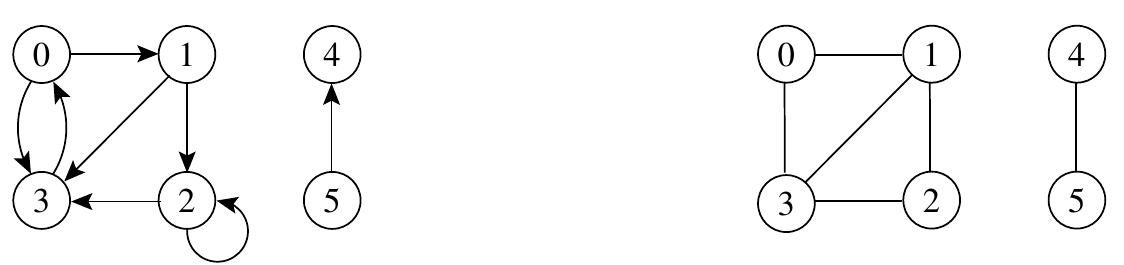
\includegraphics[width=300pt]{imagens/exemplo_versao_nao_direcionada.png}
  \label{fig_exemplo_versao_nao_direcionada}
\end{figure}
\end{frame}

%%%%%%%%%%%%%%%%%%%%%%%%%%%%%%%%%%%%%%%%%%%%%%%%%%%%%%%%%%%%%%%%%%%%%%%%%%%%%%%%%%%%%%%%%%%%%%%%%%%%%%%%%%%%%%%%%%%%%%%%%%%%%% 

\begin{frame}{Definições}{Grafo Ponderado}
\begin{itemize}
\item Um {\bf grafo ponderado} possui pesos associados às arestas.
\begin{figure}[!h]
  \centering
  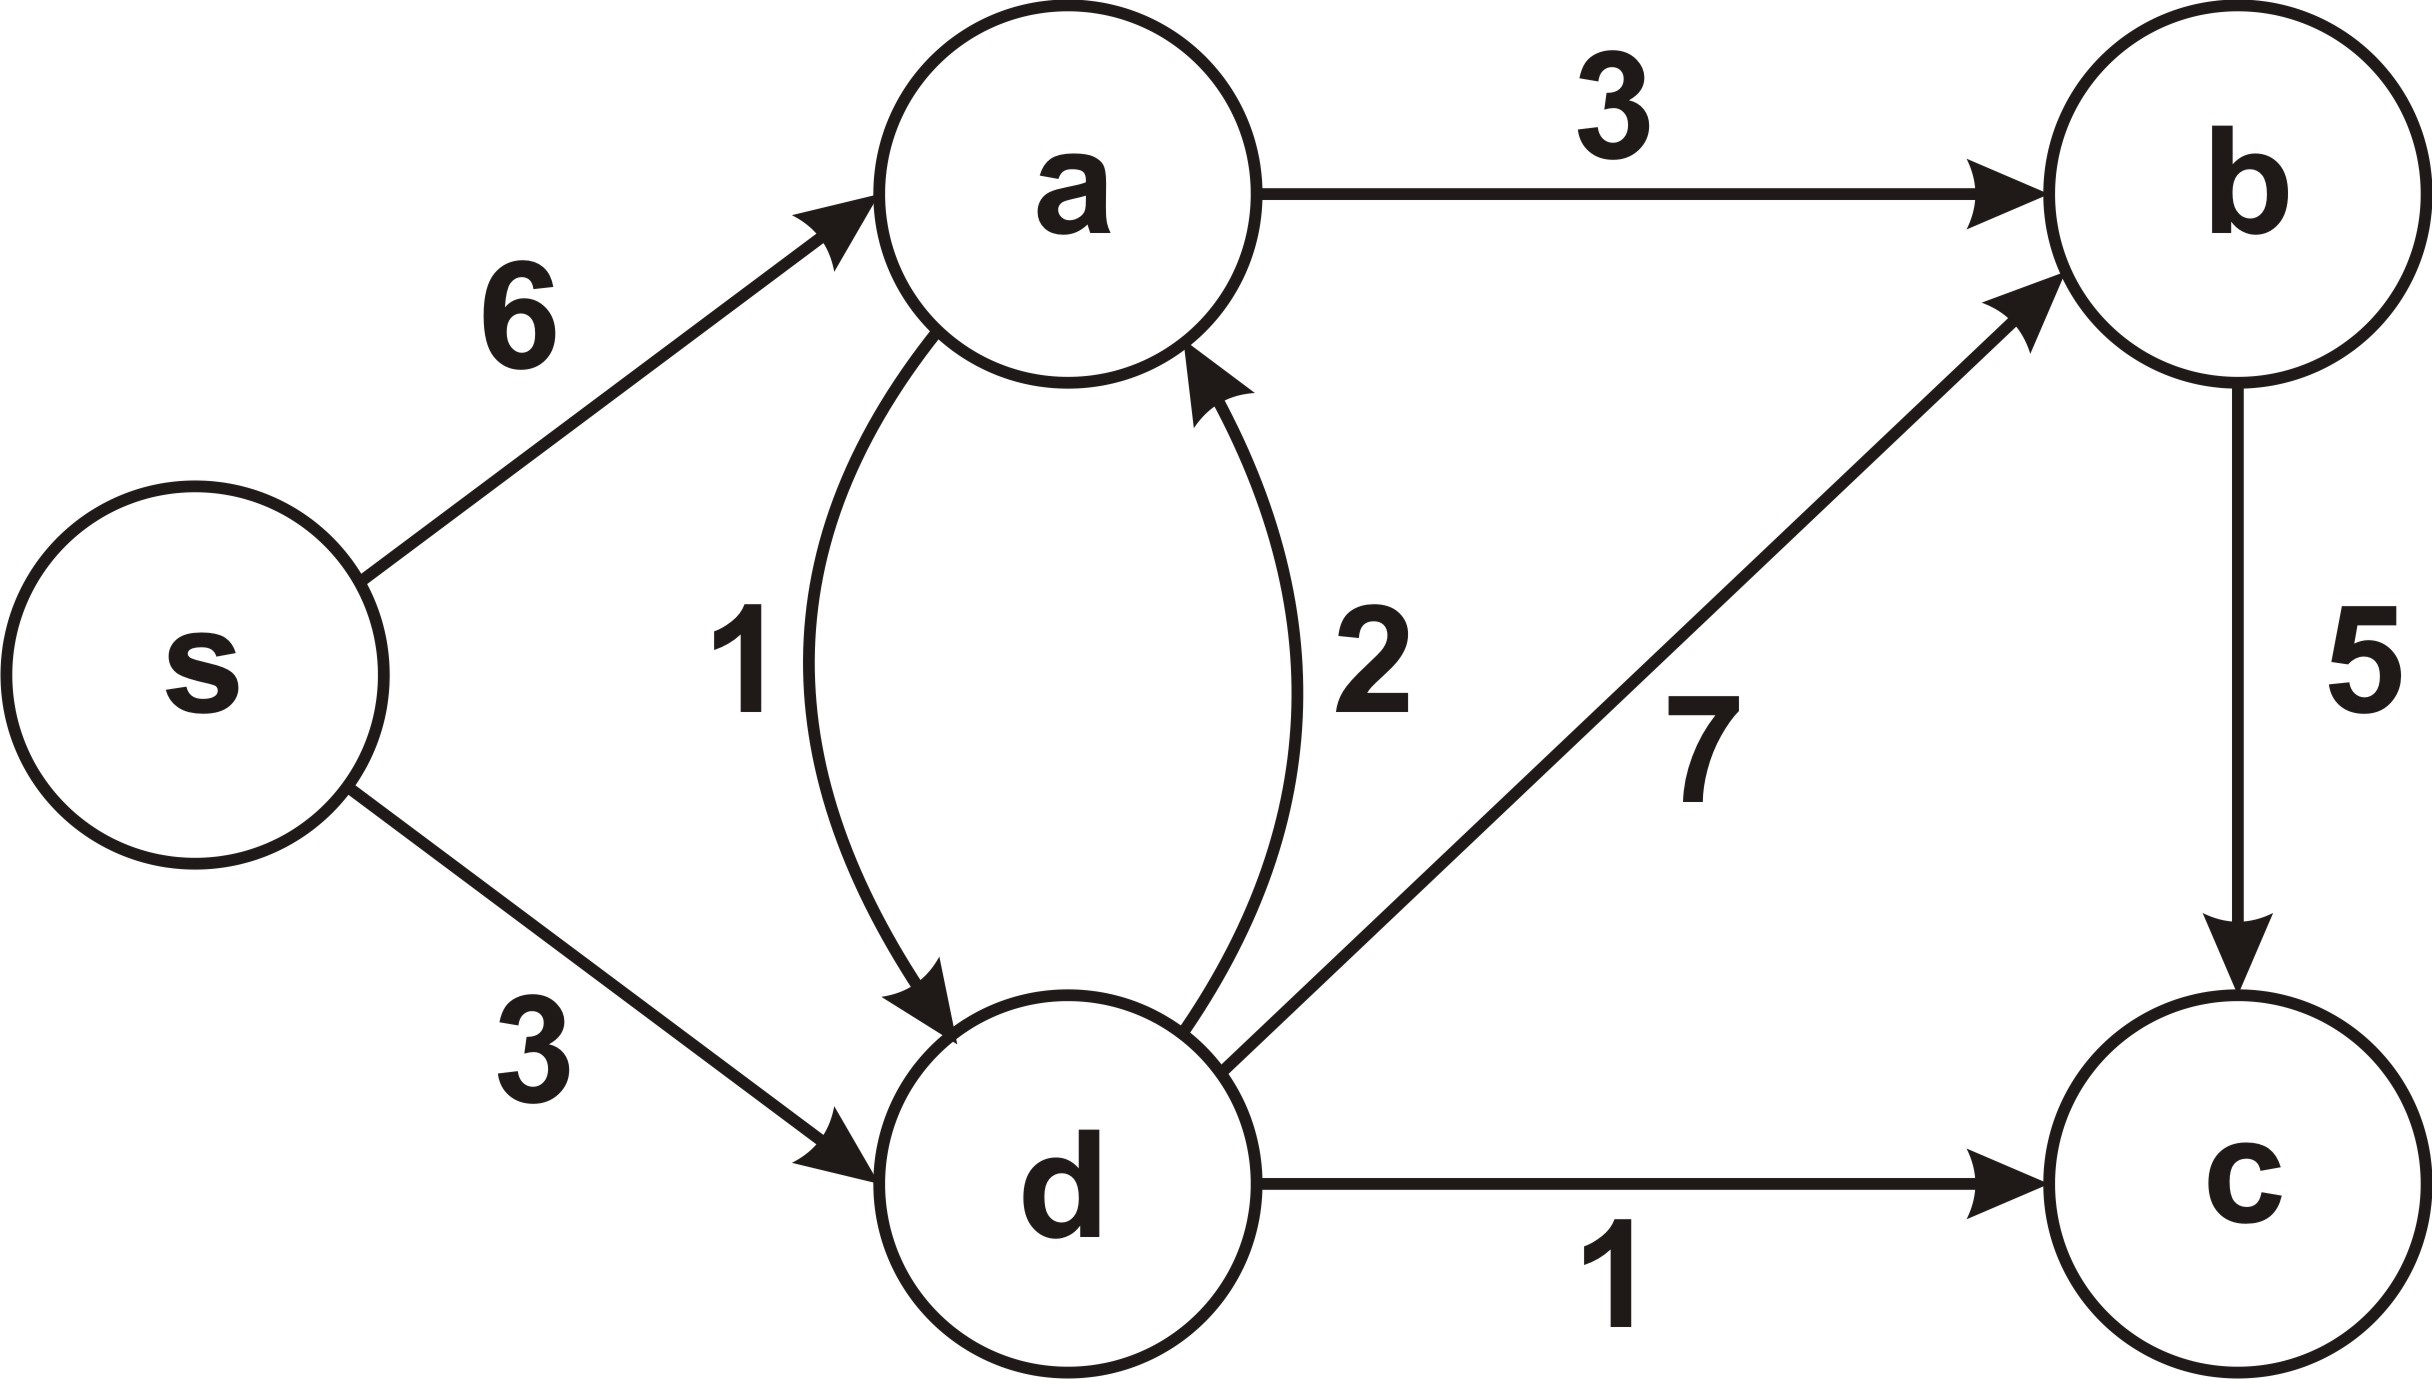
\includegraphics[width=150pt]{imagens/exemplo_grafo_ponderado.jpg}
  \label{fig_exemplo_grafo_ponderado}
\end{figure}
\end{itemize}
\end{frame}

%%%%%%%%%%%%%%%%%%%%%%%%%%%%%%%%%%%%%%%%%%%%%%%%%%%%%%%%%%%%%%%%%%%%%%%%%%%%%%%%%%%%%%%%%%%%%%%%%%%%%%%%%%%%%%%%%%%%%%%%%%%%%% 

\begin{frame}{Definições}{Grafo Bipartido}
\begin{itemize}
\item {\bf Grafo Bipartido}: grafo não-direcionado $G = (V, A)$ no qual V {\it pode ser particionado em dois conjuntos} $V_1$ e $V_2$ tal que $(u, v) \in A$ implica que $u \in V_1$ e $v \in V_2$ ou $u \in V_2$ e $v \in V_1$ (todas as arestas ligam os dois conjuntos $V_1$ e $V_2$ ).

\begin{figure}[!h]
  \centering
  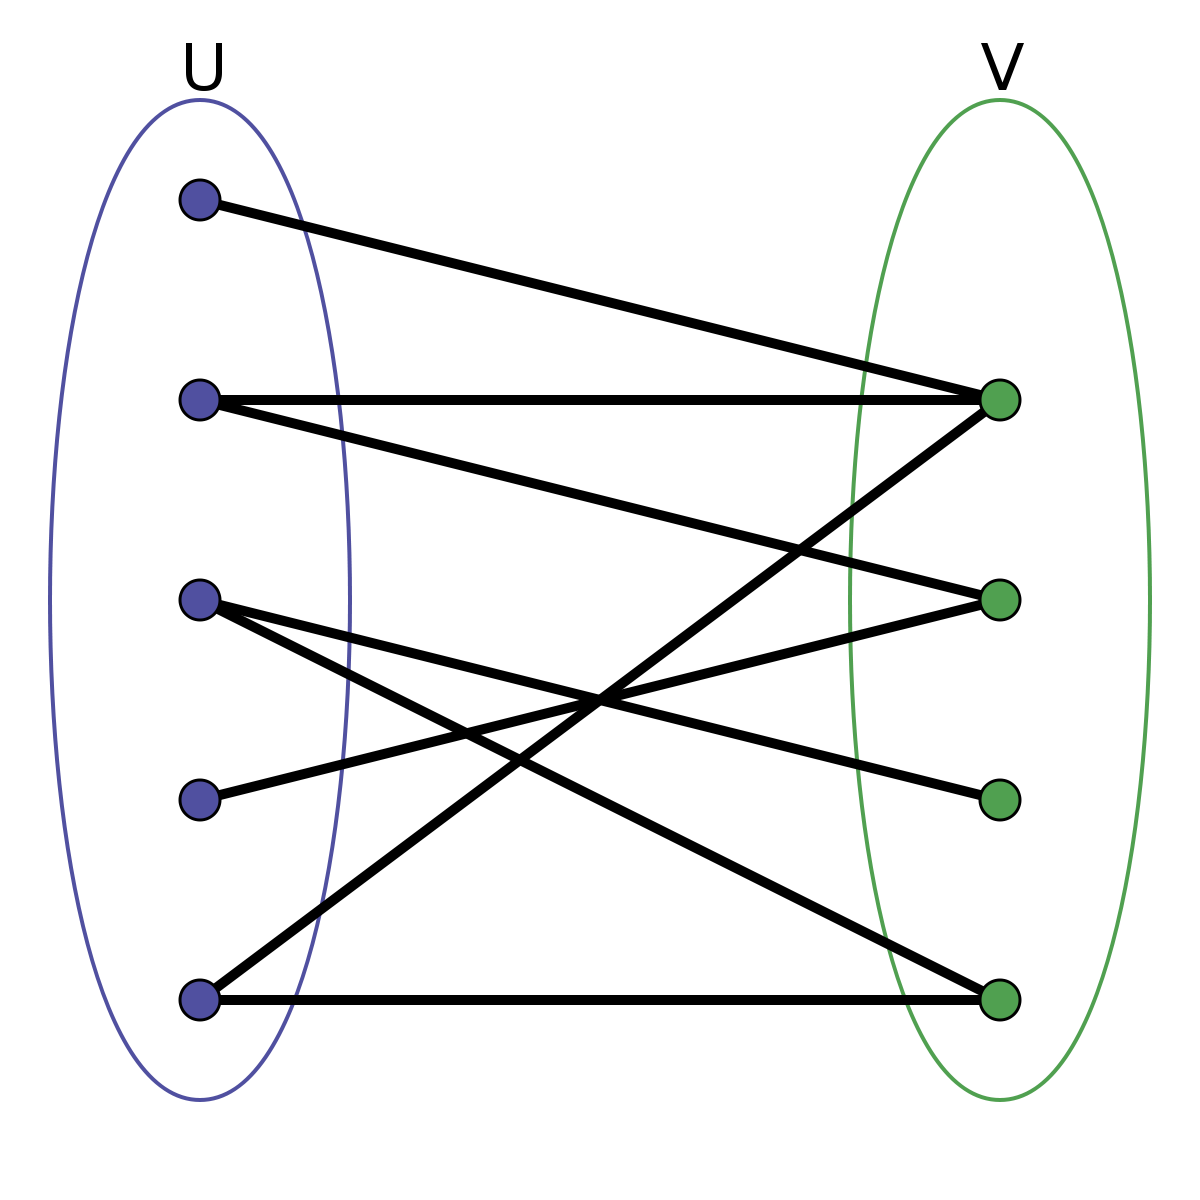
\includegraphics[width=150pt]{imagens/exemplo_grafo_bipartido.png}
  \label{fig_exemplo_grafo_bipartido}
\end{figure}
\end{itemize}
\end{frame}

%%%%%%%%%%%%%%%%%%%%%%%%%%%%%%%%%%%%%%%%%%%%%%%%%%%%%%%%%%%%%%%%%%%%%%%%%%%%%%%%%%%%%%%%%%%%%%%%%%%%%%%%%%%%%%%%%%%%%%%%%%%%%% 

\begin{frame}{Definições}{Grafo Bipartido}
\begin{figure}[!h]
  \centering
  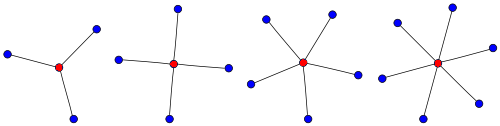
\includegraphics[width=300pt]{imagens/exemplo_grafo_bipartido1.png}
  \label{fig_exemplo_grafo_bipartido1}
\end{figure}
\end{frame}

%%%%%%%%%%%%%%%%%%%%%%%%%%%%%%%%%%%%%%%%%%%%%%%%%%%%%%%%%%%%%%%%%%%%%%%%%%%%%%%%%%%%%%%%%%%%%%%%%%%%%%%%%%%%%%%%%%%%%%%%%%%%%% 

\begin{frame}{Definições}{Grafo Bipartido}
\begin{figure}[!h]
  \centering
  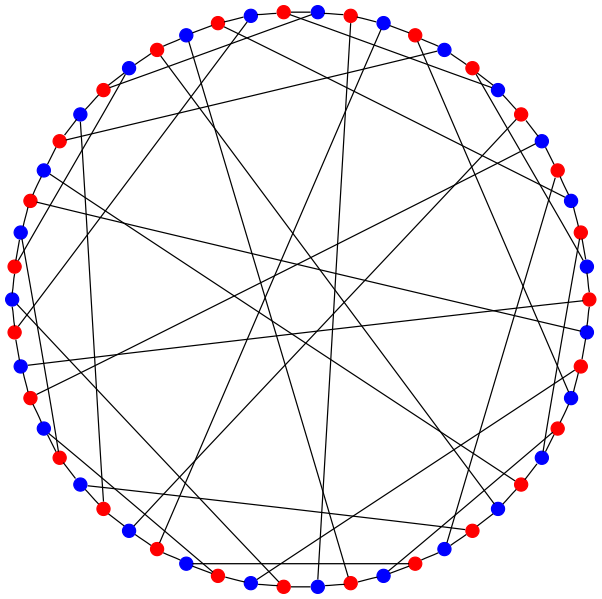
\includegraphics[width=150pt]{imagens/exemplo_grafo_bipartido2.png}
  \label{fig_exemplo_grafo_bipartido2}
\end{figure}
\end{frame}

%%%%%%%%%%%%%%%%%%%%%%%%%%%%%%%%%%%%%%%%%%%%%%%%%%%%%%%%%%%%%%%%%%%%%%%%%%%%%%%%%%%%%%%%%%%%%%%%%%%%%%%%%%%%%%%%%%%%%%%%%%%%%% 

\begin{frame}{Definições}{Grafo Bipartido}
\begin{figure}[!h]
  \centering
  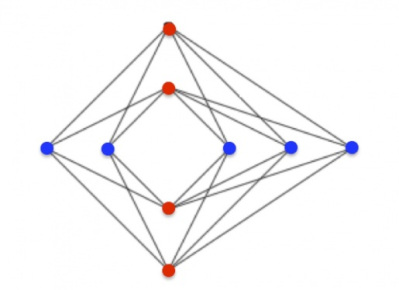
\includegraphics[width=100pt]{imagens/exemplo_grafo_bipartido3.jpg}
  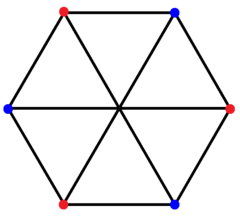
\includegraphics[width=80pt]{imagens/exemplo_grafo_bipartido4.png}
  \label{fig_exemplo_grafo_bipartido4}
\end{figure}
\begin{figure}[!h]
  \centering
  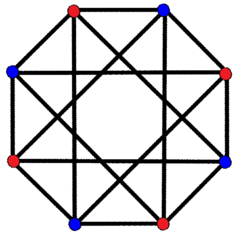
\includegraphics[width=80pt]{imagens/exemplo_grafo_bipartido5.png}
  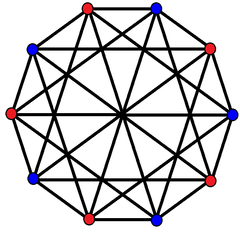
\includegraphics[width=80pt]{imagens/exemplo_grafo_bipartido6.png}
  \label{fig_exemplo_grafo_bipartido5}
\end{figure}
\end{frame}

%%%%%%%%%%%%%%%%%%%%%%%%%%%%%%%%%%%%%%%%%%%%%%%%%%%%%%%%%%%%%%%%%%%%%%%%%%%%%%%%%%%%%%%%%%%%%%%%%%%%%%%%%%%%%%%%%%%%%%%%%%%%%% 

\begin{frame}{Definições}{Grafo Tripartido}
\begin{figure}[!h]
  \centering
  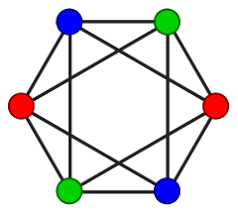
\includegraphics[width=80pt]{imagens/exemplo_grafo_tripartido.png}
  \label{fig_exemplo_grafo_tripartido}
\end{figure}
\end{frame}

%%%%%%%%%%%%%%%%%%%%%%%%%%%%%%%%%%%%%%%%%%%%%%%%%%%%%%%%%%%%%%%%%%%%%%%%%%%%%%%%%%%%%%%%%%%%%%%%%%%%%%%%%%%%%%%%%%%%%%%%%%%%%% 

\begin{frame}{Definições}{Hipergrafo}
{\bf Hipergrafo} é uma generalização de um grafo, com suas {\it arestas ligando quaisquer quantidades positivas de vértices}.
\begin{itemize}
\item {\it Definição}: Um hipergrafo $H(V,F)$ é definido pelo par de conjunto $V$ e $F$, onde:
\begin{itemize}
\item $V$ é um conjunto não vazio de vértices;
\item $F$ é um conjunto que representa uma ``família'' e partes não vazias de $V$.	
\end{itemize}
\end{itemize}
\end{frame}

%%%%%%%%%%%%%%%%%%%%%%%%%%%%%%%%%%%%%%%%%%%%%%%%%%%%%%%%%%%%%%%%%%%%%%%%%%%%%%%%%%%%%%%%%%%%%%%%%%%%%%%%%%%%%%%%%%%%%%%%%%%%%% 

\begin{frame}{Definições}{Hipergrafo}
Um {\bf hipergrafo} é um grafo não dirigido em que cada aresta conecta um número arbitrário de vértices.
\begin{itemize}
\item Seja, por exemplo, o grafo $H(V,F)$ dado por:
\begin{itemize}
\item $V =\{v_1, v_2, v_3, v_4 \}$
\item $F = \{ \{v_1, v_2, v_4 \}, {\color{blue} \{v_2, v_3, v_4 \} },{\color{red} \{v_2, v_3 \} } \}$ 
\end{itemize}
\end{itemize}
\begin{figure}[!h]
  \centering
  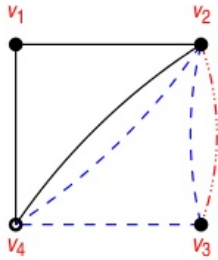
\includegraphics[width=55pt]{imagens/exemplo_hipergrafo.png}
  \label{fig_exemplo_hipergrafo}
\end{figure}
\end{frame}

%%%%%%%%%%%%%%%%%%%%%%%%%%%%%%%%%%%%%%%%%%%%%%%%%%%%%%%%%%%%%%%%%%%%%%%%%%%%%%%%%%%%%%%%%%%%%%%%%%%%%%%%%%%%%%%%%%%%%%%%%%%%%% 

\begin{frame}{Definições}{Grafos Completos}
\begin{itemize}
\item Um {\bf grafo completo} é um grafo não-direcionado no qual todos os pares de vértices são adjacentes.
\item Possui $(|V|^2 - |V|)/2 = |V|(|V| - 1)/2$ arestas, pois do total de $|V|^2$ pares possíveis de vértices devemos subtrair $|V|$ self-loops e dividir por 2 (cada aresta ligando dois vértices é contada duas vezes).
\item O número total de grafos diferentes com $|V|$ vértices é $2^{|V|(|V|-1)/2}$ (número de maneiras diferentes de escolher um subconjunto a partir de $|V|(|V| - 1)/2$ possíveis arestas).
\end{itemize}
\end{frame}

%%%%%%%%%%%%%%%%%%%%%%%%%%%%%%%%%%%%%%%%%%%%%%%%%%%%%%%%%%%%%%%%%%%%%%%%%%%%%%%%%%%%%%%%%%%%%%%%%%%%%%%%%%%%%%%%%%%%%%%%%%%%%% 

\begin{frame}{Definições}{Grafos Completos}
\begin{figure}[!h]
  \centering
  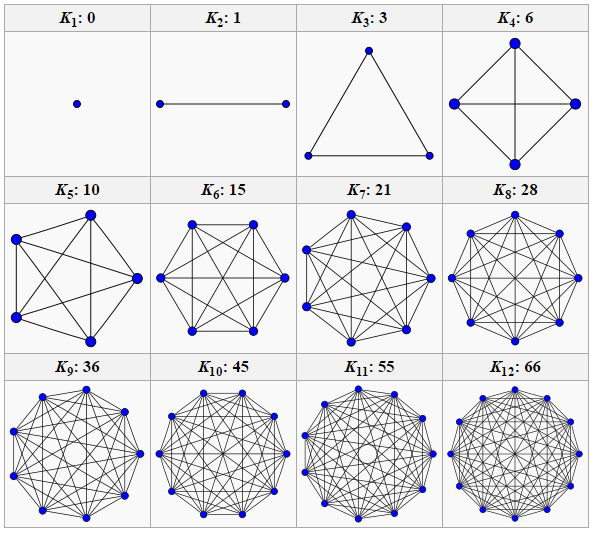
\includegraphics[width=200pt]{imagens/grafo_completo.png}
  \label{fig_exemplo_grafo_completo}
\end{figure}
\end{frame}

%%%%%%%%%%%%%%%%%%%%%%%%%%%%%%%%%%%%%%%%%%%%%%%%%%%%%%%%%%%%%%%%%%%%%%%%%%%%%%%%%%%%%%%%%%%%%%%%%%%%%%%%%%%%%%%%%%%%%%%%%%%%%% 

\begin{frame}{Definições}{Árvores}
\begin{itemize}
\item {\bf Árvore livre}: grafo não-direcionado acíclico e conectado.
\item É comum dizer apenas que o grafo é uma árvore omitindo o ``livre''.
\item {\bf Floresta}: grafo não-direcionado acíclico, podendo ou não ser
conectado.
\end{itemize}
\begin{figure}[!h]
  \centering
  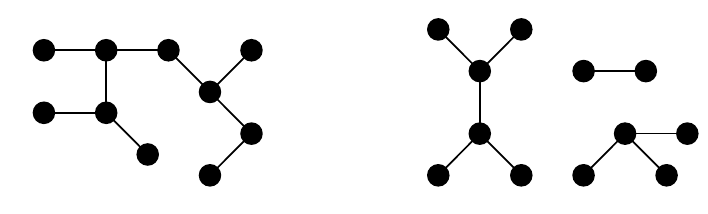
\includegraphics[width=200pt]{imagens/exemplo_arvores.png}
  \label{fig_exemplo_arvores}
\end{figure}
\end{frame}

%%%%%%%%%%%%%%%%%%%%%%%%%%%%%%%%%%%%%%%%%%%%%%%%%%%%%%%%%%%%%%%%%%%%%%%%%%%%%%%%%%%%%%%%%%%%%%%%%%%%%%%%%%%%%%%%%%%%%%%%%%%%%% 
\section{Representação}
%%%%%%%%%%%%%%%%%%%%%%%%%%%%%%%%%%%%%%%%%%%%%%%%%%%%%%%%%%%%%%%%%%%%%%%%%%%%%%%%%%%%%%%%%%%%%%%%%%%%%%%%%%%%%%%%%%%%%%%%%%%%%% 

\begin{frame}{Representação}
As principais formas para representar grafos são:
\begin{itemize}
\item {\bf Matriz de Adjacência}
\item {\bf Lista de Adjacência}
\end{itemize}
\end{frame}

%%%%%%%%%%%%%%%%%%%%%%%%%%%%%%%%%%%%%%%%%%%%%%%%%%%%%%%%%%%%%%%%%%%%%%%%%%%%%%%%%%%%%%%%%%%%%%%%%%%%%%%%%%%%%%%%%%%%%%%%%%%%%% 
\subsection{Matriz de Adjacência}
%%%%%%%%%%%%%%%%%%%%%%%%%%%%%%%%%%%%%%%%%%%%%%%%%%%%%%%%%%%%%%%%%%%%%%%%%%%%%%%%%%%%%%%%%%%%%%%%%%%%%%%%%%%%%%%%%%%%%%%%%%%%%% 

\begin{frame}{Representação}{Matriz de Adjacência}
\begin{itemize}
\item A {\bf Matriz de Adjacência} de um grafo $G = (V, A)$ contendo n vértices é uma matriz $n \times n$ de bits, onde $A[i, j]$ é $1$ (ou verdadeiro) se e somente se existe um arco do vértice $i$ para o vértice $j$.
\item Para grafos ponderados $A[i, j]$ contém o rótulo ou peso associado com a aresta e, neste caso, a matriz não é de bits.
\item Se não existir uma aresta de $i$ para $j$ então é necessário utilizar um valor que não possa ser usado como rótulo ou peso.
\end{itemize}
\end{frame}

%%%%%%%%%%%%%%%%%%%%%%%%%%%%%%%%%%%%%%%%%%%%%%%%%%%%%%%%%%%%%%%%%%%%%%%%%%%%%%%%%%%%%%%%%%%%%%%%%%%%%%%%%%%%%%%%%%%%%%%%%%%%%% 

\begin{frame}{Representação}{Matriz de Adjacência}
\begin{figure}[!h]
  \centering
  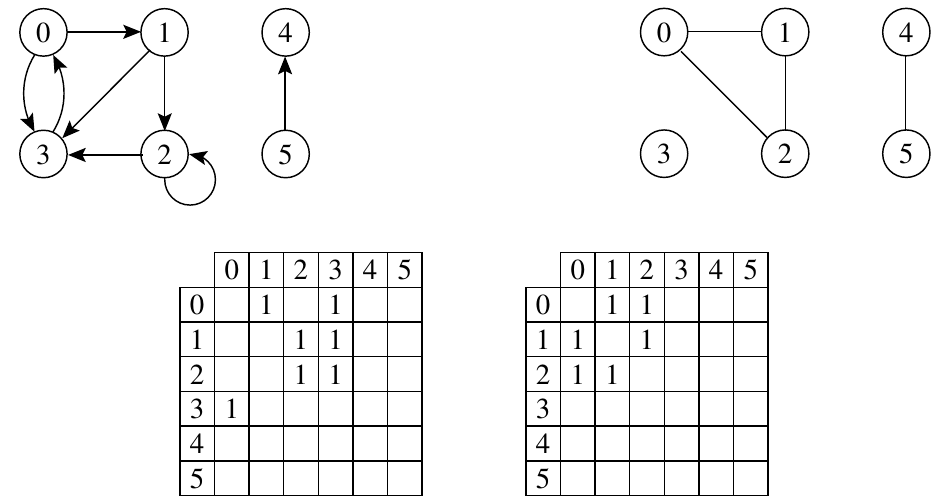
\includegraphics[width=300pt]{imagens/exemplo_matriz_adjacencia.png}
  \label{fig_exemplo_matriz_adjacencia}
\end{figure}
\end{frame}

%%%%%%%%%%%%%%%%%%%%%%%%%%%%%%%%%%%%%%%%%%%%%%%%%%%%%%%%%%%%%%%%%%%%%%%%%%%%%%%%%%%%%%%%%%%%%%%%%%%%%%%%%%%%%%%%%%%%%%%%%%%%%% 

\begin{frame}{Matriz de Adjacência}{Análise}
\begin{itemize}
\item Deve ser utilizada para grafos densos, onde $|A|$ é próximo de $|V|^2$ .
\item {\color{blue} Vantagens}:
\begin{itemize}
\item O tempo necessário para acessar um elemento é independente de $|V|$ ou $|A|$.
\item É muito útil para algoritmos em que necessitamos saber com rapidez se existe uma aresta ligando dois vértices.
\end{itemize}
\item {\color{red} Desvantagens}:
\begin{itemize}
\item A maior desvantagem é que a matriz necessita $\omega(|V|^2)$ de espaço. 
\item Ler ou examinar a matriz tem complexidade de tempo $O(|V|^2 )$.
\end{itemize}
\end{itemize}
\end{frame}

%%%%%%%%%%%%%%%%%%%%%%%%%%%%%%%%%%%%%%%%%%%%%%%%%%%%%%%%%%%%%%%%%%%%%%%%%%%%%%%%%%%%%%%%%%%%%%%%%%%%%%%%%%%%%%%%%%%%%%%%%%%%%% 
\subsection{Lista de Adjacência}
%%%%%%%%%%%%%%%%%%%%%%%%%%%%%%%%%%%%%%%%%%%%%%%%%%%%%%%%%%%%%%%%%%%%%%%%%%%%%%%%%%%%%%%%%%%%%%%%%%%%%%%%%%%%%%%%%%%%%%%%%%%%%% 

\begin{frame}{Representação}{Lista de Adjacência}
\begin{itemize}
\item A {\bf Lista de Adjacência} consiste de um vetor, denominado $Adj$, contendo $|V|$ listas, uma para cada vértice de $V$.
\item Para cada $u \in V$, Adj[u] contém todos os vértices de $G$ adjacentes a $u$.
\item Os vértices são armazenados de forma arbitrária na lista.
\item Também pode ser utilizada para representar grafos dirigidos.
\end{itemize}
\end{frame}

%%%%%%%%%%%%%%%%%%%%%%%%%%%%%%%%%%%%%%%%%%%%%%%%%%%%%%%%%%%%%%%%%%%%%%%%%%%%%%%%%%%%%%%%%%%%%%%%%%%%%%%%%%%%%%%%%%%%%%%%%%%%%% 

\begin{frame}{Representação}{Lista de Adjacência}
\begin{figure}[!h]
  \centering
  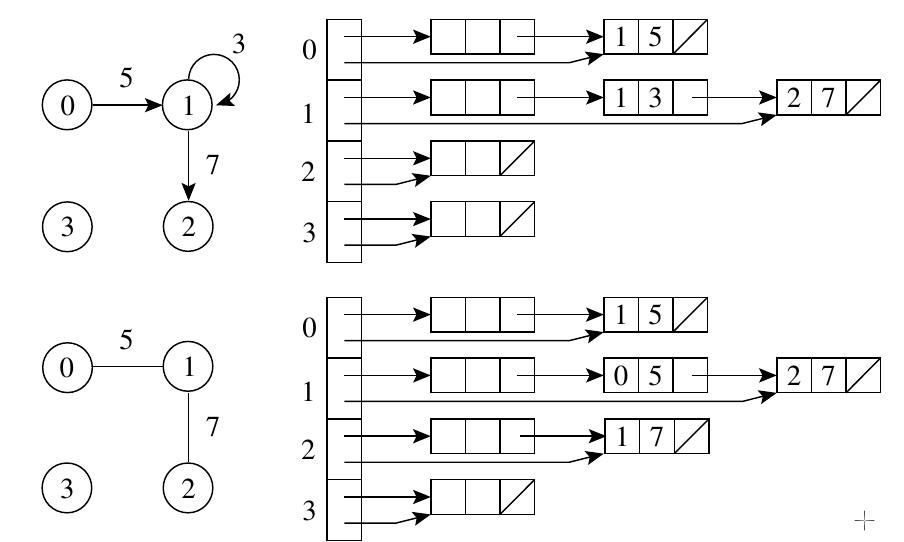
\includegraphics[width=300pt]{imagens/exemplo_lista_adjacencia.png}
  \label{fig_exemplo_lista_adjacencia}
\end{figure}
\end{frame}

%%%%%%%%%%%%%%%%%%%%%%%%%%%%%%%%%%%%%%%%%%%%%%%%%%%%%%%%%%%%%%%%%%%%%%%%%%%%%%%%%%%%%%%%%%%%%%%%%%%%%%%%%%%%%%%%%%%%%%%%%%%%%% 

\begin{frame}{Lista de Adjacência}{Análise}
\begin{itemize}
\item Os vértices de uma lista de adjacência são em geral armazenados em uma ordem arbitrária.
\item Indicada para grafos esparsos, onde $|A|$ é muito menor do que $|V|^2$.
\item {\color{blue} Vantagens}:
\begin{itemize}
\item É compacta e usualmente utilizada na maioria das aplicações.
\item Possui uma complexidade de espaço $O(|V| + |A|)$.
\end{itemize}
\item {\color{red} Desvantagens}:
\begin{itemize}
\item É ineficiente para determinar se uma aresta está no grafo.
\item A principal desvantagem é que ela pode ter tempo $O(|V|)$ para determinar se existe uma aresta entre o vértice $i$ e o vértice $j$, pois
podem existir $O(|V|)$ vértices na lista de adjacentes do vértice $i$.
\end{itemize}
\end{itemize}
\end{frame}

%%%%%%%%%%%%%%%%%%%%%%%%%%%%%%%%%%%%%%%%%%%%%%%%%%%%%%%%%%%%%%%%%%%%%%%%%%%%%%%%%%%%%%%%%%%%%%%%%%%%%%%%%%%%%%%%%%%%%%%%%%%%%% 
\section{Percurso}
%%%%%%%%%%%%%%%%%%%%%%%%%%%%%%%%%%%%%%%%%%%%%%%%%%%%%%%%%%%%%%%%%%%%%%%%%%%%%%%%%%%%%%%%%%%%%%%%%%%%%%%%%%%%%%%%%%%%%%%%%%%%%% 

\begin{frame}{Percurso}
\begin{itemize}
\item Fazer buscas em um grafo significa percorrer suas arestas sistematicamente, de modo a visitar seus vértices.
\item As principais formas para percorrer grafos são:
\begin{itemize}
\item {\bf Busca em Largura} - em inglês {\it Breadth-First Search} ou BFS
\item {\bf Busca em Profundidade} - em inglês {\it Depth-First Search} ou DFS
\end{itemize}
\end{itemize}
\end{frame}

%%%%%%%%%%%%%%%%%%%%%%%%%%%%%%%%%%%%%%%%%%%%%%%%%%%%%%%%%%%%%%%%%%%%%%%%%%%%%%%%%%%%%%%%%%%%%%%%%%%%%%%%%%%%%%%%%%%%%%%%%%%%%% 
\subsection{Busca em Largura}
%%%%%%%%%%%%%%%%%%%%%%%%%%%%%%%%%%%%%%%%%%%%%%%%%%%%%%%%%%%%%%%%%%%%%%%%%%%%%%%%%%%%%%%%%%%%%%%%%%%%%%%%%%%%%%%%%%%%%%%%%%%%%% 

\begin{frame}{Percurso}{Busca em Largura}
\begin{itemize}
\item A {\bf Busca em Largura} é um dos algoritmos mais simples para exploração de um grafo.
\begin{itemize}
\item Dados um grafo G = (V, E) e um vértice $s$, chamado de fonte, a busca em largura sistematicamente explora as arestas de $G$ de maneira a visitar todos os vértices alcançáveis a partir de $s$.
\end{itemize}
\item  Expande a fronteira entre vértices descobertos e não-descobertos uniformemente através da largura da fronteira.
  \begin{itemize}
  \item O algoritmo descobre todos os vértices a uma distância $k$ do vértice de origem $s$ antes de descobrir qualquer vértice a uma distância $k + 1$.
  \end{itemize}
\item O grafo pode ser direcionado ou não-direcionado.
\end{itemize}
\end{frame}

%%%%%%%%%%%%%%%%%%%%%%%%%%%%%%%%%%%%%%%%%%%%%%%%%%%%%%%%%%%%%%%%%%%%%%%%%%%%%%%%%%%%%%%%%%%%%%%%%%%%%%%%%%%%%%%%%%%%%%%%%%%%%% 

\begin{frame}{Percurso}{Busca em Largura}
 Esse algoritmo é base para muitos outros algoritmos, como por exemplo:
\begin{itemize}
\item Achar componentes conectados.
\item Achar todos os nós contectados a apenas um nó.
\item Achar o menor caminho entre um nó raiz e os outros nós do grafo (algoritmo de Dijsktra).
\item Testar bipartição em grafos.

\end{itemize}
\end{frame}

%%%%%%%%%%%%%%%%%%%%%%%%%%%%%%%%%%%%%%%%%%%%%%%%%%%%%%%%%%%%%%%%%%%%%%%%%%%%%%%%%%%%%%%%%%%%%%%%%%%%%%%%%%%%%%%%%%%%%%%%%%%%%% 

\begin{frame}{Busca em Largura}{Algoritmo}
%\scalebox{0.65}{
\begin{algorithm}[H]
\caption{BFS} 
\label{BuscaEmLarguraIdeia}
\Entrada{Grafo $G = (V,A)$, vértice inicial $s$.}
\Inicio{
  Marque $s$ como explorado. \\
  Imprima($s$).\\  
  Enfileire-o em Q. \\
  \Enqto{($Q$ não estiver vazia)} {
    Desenfileira o 1º vértice $u$ em Q. \\
    \Para {cada vértice $v$ vizinho de $u$} {
      \Se{$v$ não foi explorado} {
		Marque $v$ como explorado. \\
		Imprima($u$).\\
		Enfileira $v$ em Q. \\
      }
    }
  }
}
\end{algorithm}
%}  
\end{frame}

%%%%%%%%%%%%%%%%%%%%%%%%%%%%%%%%%%%%%%%%%%%%%%%%%%%%%%%%%%%%%%%%%%%%%%%%%%%%%%%%%%%%%%%%%%%%%%%%%%%%%%%%%%%%%%%%%%%%%%%%%%%%%% 

\begin{frame}{Percurso}{Busca em Largura}
Algoritmo:
\begin{itemize}
\item Para controlar a busca, o algoritmo da Busca em Largura pinta cada vértice na cor branca, cinza ou preto.
\item Todos os vértices iniciam com a cor branca e podem, mais tarde, se tornar cinza e depois preto.
\begin{itemize}
\item Branca: não visitado;
\item Cinza: visitado;
\item Preta: visitado e seus nós adjacentes visitados.
\end{itemize}
\end{itemize}
\end{frame}

%%%%%%%%%%%%%%%%%%%%%%%%%%%%%%%%%%%%%%%%%%%%%%%%%%%%%%%%%%%%%%%%%%%%%%%%%%%%%%%%%%%%%%%%%%%%%%%%%%%%%%%%%%%%%%%%%%%%%%%%%%%%%% 

\begin{frame}{Percurso}{Busca em Largura}
\begin{figure}[!h]
  \centering
  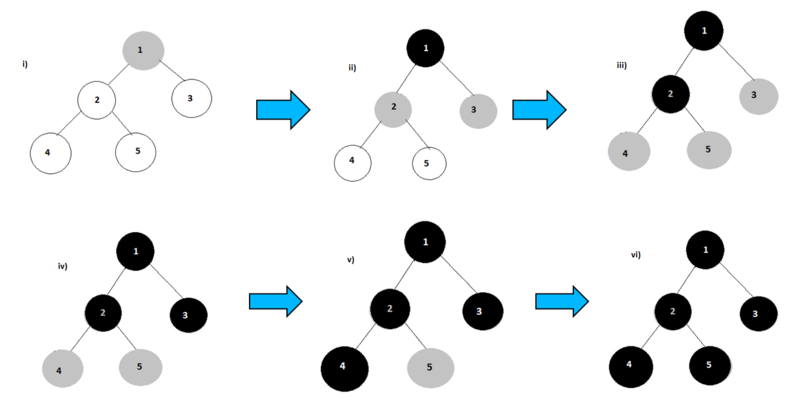
\includegraphics[width=300pt]{imagens/breadth_first_search.png}
  \label{fig_breadth_first_search}
\end{figure}
\end{frame}

%%%%%%%%%%%%%%%%%%%%%%%%%%%%%%%%%%%%%%%%%%%%%%%%%%%%%%%%%%%%%%%%%%%%%%%%%%%%%%%%%%%%%%%%%%%%%%%%%%%%%%%%%%%%%%%%%%%%%%%%%%%%%% 

\begin{frame}{Percurso}{Busca em Largura}
\begin{itemize}
\item Dado um nó inicial $s$, a busca em largura determina a distância (em número de arestas) de cada vértice atingível a partir de $s$.
\begin{itemize}
\item Vértices a uma distância de $k+1$ arestas de $s$ só são visitados após todos os vértices a uma distância de $k$ terem sido visitados.
\end{itemize}
\item Para isso, armazena em cada vértice com a distância $d$ do vértice inicial $s$.
\item Também armazena em cada vértice o seu predecessor $\pi$, exceto o vértice inicial, que não possui predecessor.
\end{itemize}
\end{frame}

%%%%%%%%%%%%%%%%%%%%%%%%%%%%%%%%%%%%%%%%%%%%%%%%%%%%%%%%%%%%%%%%%%%%%%%%%%%%%%%%%%%%%%%%%%%%%%%%%%%%%%%%%%%%%%%%%%%%%%%%%%%%%% 

\begin{frame}{Percurso}{Busca em Largura}
\scalebox{0.65}{
\begin{algorithm}[H]
\caption{BuscaEmLargura} 
\label{BuscaEmLargura}
\Entrada{Grafo $G = (V,A)$, vértice inicial $s$.}
\Saida{Percurso armazenado no campo ``predecessor'' presente em cada vértice $v \in V$.}
\Inicio{
  \Para {cada vértice $v \in V$} {
    v.$cor \leftarrow$ Branco \\
    v.$d \leftarrow \infty$ \\ 
    v.$\pi \leftarrow$ NULL \\
  }
  s.$cor \leftarrow$ Cinza \\
  s.$d \leftarrow$ 0 \\
  s.$\pi \leftarrow$ NULL \\
  CriaFilaVazia(Q) \\
  Enfileira(Q, s) \\
  \Enqto{($Q \neq \emptyset$)} {
    v $\leftarrow$ Desenfileira(Q) \\
    \Para {cada vértice $u \in v.ListaAdj$} {
      \Se{u.cor = Branco} {
			u.cor $\leftarrow$ Cinza \\
			u.d $\leftarrow$ v.d + 1 \\
			u.$\pi \leftarrow$ v \\
			Enfileira(Q, u)\\
      }
    }
    v.cor $\leftarrow$ Preto \\
  }
}
\end{algorithm}
}  
\tiny{Adaptado de \citeonline{Cormen2012}.}
\end{frame}

%%%%%%%%%%%%%%%%%%%%%%%%%%%%%%%%%%%%%%%%%%%%%%%%%%%%%%%%%%%%%%%%%%%%%%%%%%%%%%%%%%%%%%%%%%%%%%%%%%%%%%%%%%%%%%%%%%%%%%%%%%%%%% 

\begin{frame}{Percurso}{Busca em Largura}
\begin{figure}[!h]
  \centering
  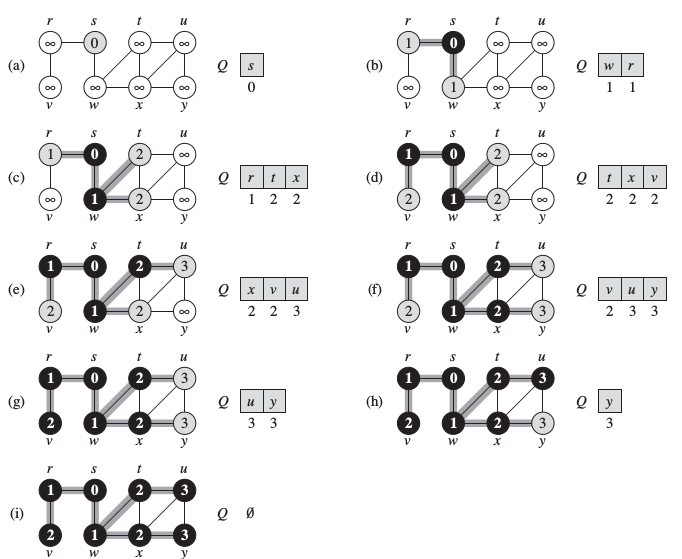
\includegraphics[width=250pt]{imagens/BFS_cormen.png}
  \label{fig_bfs_cormen}
\end{figure}
\end{frame}

%%%%%%%%%%%%%%%%%%%%%%%%%%%%%%%%%%%%%%%%%%%%%%%%%%%%%%%%%%%%%%%%%%%%%%%%%%%%%%%%%%%%%%%%%%%%%%%%%%%%%%%%%%%%%%%%%%%%%%%%%%%%%% 

\begin{frame}{Busca em Largura}{Análise}
\begin{itemize}
\item Uma característica do BFS é que sua árvore de busca resultante corresponde ao {\it caminho mais curto} do vértice inicial a qualquer vértice do grafo.
\item Cada vértice de $V$ é colocado na fila $Q$ no máximo uma vez: $O(V)$;
\item A lista de adjacência de um vértice qualquer de $u$ é percorrida somente quando o vértice é removido da fila;
\item A soma de todas as listas de adjacentes é $O(A)$, então o tempo total gasto com as listas de adjacentes é $O(A)$;
\item Enfileirar e desenfileirar tem custo $O(1)$;
\item Complexidade: $O(V + A)$.
\end{itemize}
\end{frame}

%%%%%%%%%%%%%%%%%%%%%%%%%%%%%%%%%%%%%%%%%%%%%%%%%%%%%%%%%%%%%%%%%%%%%%%%%%%%%%%%%%%%%%%%%%%%%%%%%%%%%%%%%%%%%%%%%%%%%%%%%%%%%% 
\subsection{Busca em Profundidade}
%%%%%%%%%%%%%%%%%%%%%%%%%%%%%%%%%%%%%%%%%%%%%%%%%%%%%%%%%%%%%%%%%%%%%%%%%%%%%%%%%%%%%%%%%%%%%%%%%%%%%%%%%%%%%%%%%%%%%%%%%%%%%% 

\begin{frame}{Percurso}{Busca em Profundidade}
\begin{itemize}
\item Na {\bf Busca em Profundidade}, a estratégia é buscar o vértice mais profundo no grafo sempre que possível:
\begin{itemize}
\item As arestas são exploradas a partir do vértice $v$ mais recentemente descoberto que ainda possui arestas não exploradas saindo dele.
\end{itemize}
\item Quando todas as arestas adjacentes a v tiverem sido exploradas a busca anda para trás para explorar vértices que
saem do vértice do qual $v$ foi descoberto ({\it backtracking}).
\end{itemize}
\end{frame}

%%%%%%%%%%%%%%%%%%%%%%%%%%%%%%%%%%%%%%%%%%%%%%%%%%%%%%%%%%%%%%%%%%%%%%%%%%%%%%%%%%%%%%%%%%%%%%%%%%%%%%%%%%%%%%%%%%%%%%%%%%%%%% 

\begin{frame}{Percurso}{Busca em Profundidade}
O algoritmo é a base para muitos outros algoritmos importantes, tais como:
\begin{itemize}
\item Verificação de grafos acíclicos, 
\item Ordenação topológica e 
\item Componentes fortemente conectados.
\item Resolução de quebra-cabeças como labirinto.
\end{itemize} 
\end{frame}

%%%%%%%%%%%%%%%%%%%%%%%%%%%%%%%%%%%%%%%%%%%%%%%%%%%%%%%%%%%%%%%%%%%%%%%%%%%%%%%%%%%%%%%%%%%%%%%%%%%%%%%%%%%%%%%%%%%%%%%%%%%%%% 

\begin{frame}{Busca em Profundidade}{Algoritmo}
%\scalebox{0.65}{
\begin{algorithm}[H]
\caption{DFS} 
\label{BuscaEmProfundidadeIdeia}
\Entrada{Grafo $G = (V,A)$, vértice inicial $v$.}
\Saida{Imprime o conteúdo de todos os vértices.}
\Inicio{
  Marque $v$ como explorado. \\
  Imprima($v$).\\
    \Para {cada vértice $u$ vizinho de $v$} {
      \Se{$u$ não foi explorado} {
		DFS(G,u).
      }
    }
  }
%}
\end{algorithm}
%}  

\tiny{Adaptado de \citeonline{Oliveira2011}.}
\end{frame}

%%%%%%%%%%%%%%%%%%%%%%%%%%%%%%%%%%%%%%%%%%%%%%%%%%%%%%%%%%%%%%%%%%%%%%%%%%%%%%%%%%%%%%%%%%%%%%%%%%%%%%%%%%%%%%%%%%%%%%%%%%%%%% 

\begin{frame}{Busca em Profundidade}{Algoritmo}
%\scalebox{0.65}{
\begin{algorithm}[H]
\caption{DFS-Não-Recursivo} 
\label{BuscaEmProfundidadeIdeiaNaoRecursivo}
\Entrada{Grafo $G = (V,A)$, vértice inicial $v$.}
\Saida{Imprime o conteúdo de todos os vértices.}
\Inicio{
  Empilhe $v$ na pilha $S$. \\
  \Enqto {$S$ não estiver vazia} {
  	Desempilhe $v$ de $S$. \\
   	Marque $v$ como explorado. \\
    \Para {cada vértice $u$ vizinho de $v$} {
      \Se{$u$ não foi explorado} {
      	Marque $u$ como explorado. \\
		Empilhe $u$ em $S$.\\
      }
    }
    \Se{$v$ não foi explorado}{
    Imprima(v).
    }
   }
  }
%}
\end{algorithm}
%}  

\tiny{Adaptado de \citeonline{Oliveira2011}.}
\end{frame}

%%%%%%%%%%%%%%%%%%%%%%%%%%%%%%%%%%%%%%%%%%%%%%%%%%%%%%%%%%%%%%%%%%%%%%%%%%%%%%%%%%%%%%%%%%%%%%%%%%%%%%%%%%%%%%%%%%%%%%%%%%%%%% 

\begin{frame}{Percurso}{Busca em Profundidade}
Algoritmo
\begin{itemize}
\item Para controlar a busca, o algoritmo da Busca em Profundidade pinta cada vértice na cor branca, cinza ou preto.
\item Todos os vértices iniciam com a cor branca e podem, mais tarde, se tornar cinza e depois preto.
\begin{itemize}
\item Branca: não visitado;
\item Cinza: visitado;
\item Preta: visitado e seus nós adjacentes visitados.
\end{itemize}
\end{itemize}
\end{frame}

%%%%%%%%%%%%%%%%%%%%%%%%%%%%%%%%%%%%%%%%%%%%%%%%%%%%%%%%%%%%%%%%%%%%%%%%%%%%%%%%%%%%%%%%%%%%%%%%%%%%%%%%%%%%%%%%%%%%%%%%%%%%%% 

\begin{frame}{Percurso}{Busca em Profundidade}
\begin{figure}[!h]
  \centering
  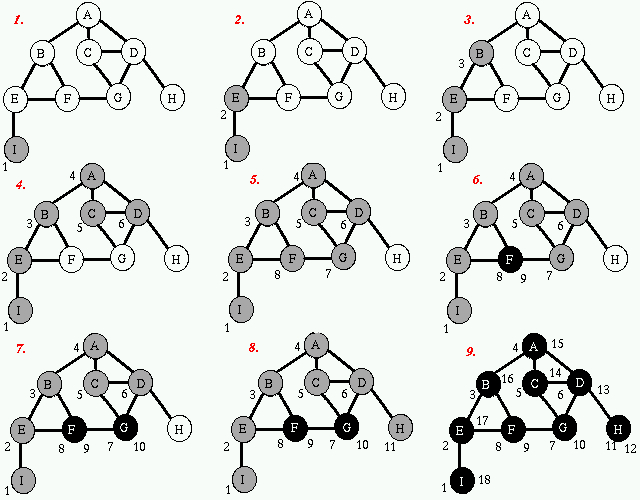
\includegraphics[width=250pt]{imagens/depth_first_search.jpg}
  \label{fig_depth_first_search}
\end{figure}
\end{frame}

%%%%%%%%%%%%%%%%%%%%%%%%%%%%%%%%%%%%%%%%%%%%%%%%%%%%%%%%%%%%%%%%%%%%%%%%%%%%%%%%%%%%%%%%%%%%%%%%%%%%%%%%%%%%%%%%%%%%%%%%%%%%%% 

\begin{frame}{Percurso}{Busca em Profundidade}
Algoritmo
\begin{itemize}
\item A busca em profundidade também marca cada vértice com um {\it timestamp}.
\item Cada vértice tem dois {\it timestamp}:
\begin{itemize}
\item v.d: indica o instante em que $v$ foi visitado (pintado com cinza);
\item v.f: indica o instante em que a busca pelos vértices na lista de adjacência de $v$ foi completada (pintado de preto).
\end{itemize}
\end{itemize}
\end{frame}

%%%%%%%%%%%%%%%%%%%%%%%%%%%%%%%%%%%%%%%%%%%%%%%%%%%%%%%%%%%%%%%%%%%%%%%%%%%%%%%%%%%%%%%%%%%%%%%%%%%%%%%%%%%%%%%%%%%%%%%%%%%%%% 

\begin{frame}{Percurso}{Busca em Profundidade}
\begin{columns}
\begin{column}{0.5\textwidth}
  \scalebox{0.8}{
  \begin{algorithm}[H]
  \caption{BuscaEmProfundidade} 
  \label{BuscaEmprofundidade}
  \Entrada{Grafo $G = (V,A)$.}
  \Saida{Percurso armazenado no campo ``predecessor'' presente em cada vértice $v \in V$.}
  \Inicio{
    \Para {cada vértice $u \in V$} {
      $u.cor \leftarrow$ Branco \\
      $u.\pi \leftarrow$ NULL \\
    }
    tempo $\leftarrow$ 0\\
    \Para {cada vértice $u \in V$} { 
      \Se {u.cor = Branco} {
		DFS-Visita(u)\\
      }
    }
  }
  \end{algorithm}
  }
\end{column}
\begin{column}{0.5\textwidth}  
    \begin{center}
  \scalebox{0.8}{
  \begin{algorithm}[H]
  \caption{DFS-Visita} 
  \label{Visita}
  \Entrada{Grafo $G = (V,A)$, vértice inicial $s$.}
  % \Saida{Percurso armazenado no campo ``predecessor'' presente em cada vértice $v \in V$.}
  \Inicio{
    tempo $\leftarrow$ tempo + 1\\
    $u.d \leftarrow$ tempo \\      
    $u.cor \leftarrow$ Cinza \\
    \Para {cada vértice $v \in u.ListaAdj$} { 
      \Se {v.cor = Branco} {
		$v.\pi \leftarrow u$ \\
		DFS-Visita(G, v)\\
      }
    }
    u.cor $\leftarrow$ Preto \\
    tempo $\leftarrow$ tempo + 1\\
    u.f $\leftarrow$ tempo \\
  }
  \end{algorithm}
  }  
     \end{center}
\end{column}
\end{columns}
\tiny{Adaptado de \citeonline{Cormen2012}.}
\end{frame}

%%%%%%%%%%%%%%%%%%%%%%%%%%%%%%%%%%%%%%%%%%%%%%%%%%%%%%%%%%%%%%%%%%%%%%%%%%%%%%%%%%%%%%%%%%%%%%%%%%%%%%%%%%%%%%%%%%%%%%%%%%%%%% 

\begin{frame}{Percurso}{Busca em Profundidade}
\begin{figure}[!h]
  \centering
  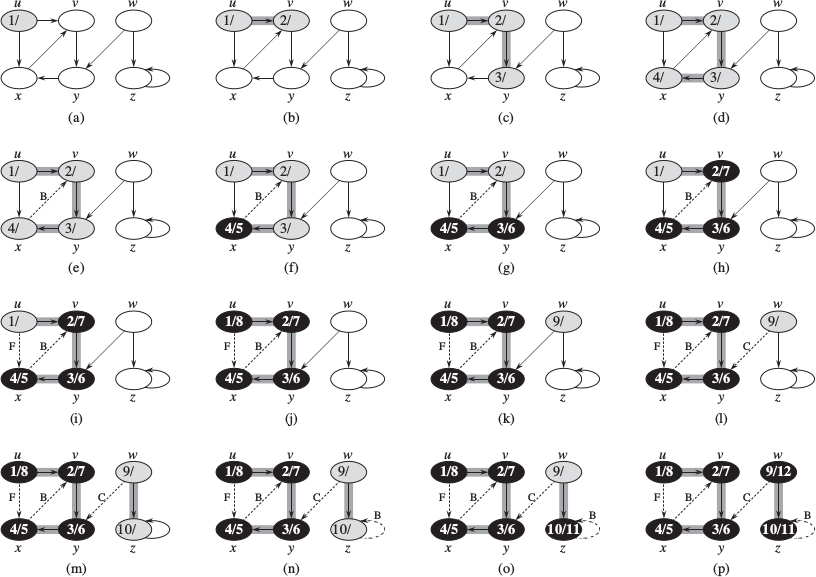
\includegraphics[width=280pt]{imagens/DFS_cormen.png}
  \label{fig_dfs_cormen}
\end{figure}
\end{frame}

%%%%%%%%%%%%%%%%%%%%%%%%%%%%%%%%%%%%%%%%%%%%%%%%%%%%%%%%%%%%%%%%%%%%%%%%%%%%%%%%%%%%%%%%%%%%%%%%%%%%%%%%%%%%%%%%%%%%%%%%%%%%%% 

\begin{frame}{Busca em Profundidade}{Análise}
\begin{itemize}
\item O procedimento DFS-Visita é chamado exatamente uma vez para cada vértice $u \in V$.
\item Isso ocorre porque DFS-Visita é chamado apenas para vértices brancos e a primeira ação é pintar o vértice de cinza: $O(V)$.
\item O loop principal de DFS-Visita ($u$) tem complexidade $O(A)$.
\item Complexidade: $O(V + A)$.
\end{itemize}
\end{frame}

%%%%%%%%%%%%%%%%%%%%%%%%%%%%%%%%%%%%%%%%%%%%%%%%%%%%%%%%%%%%%%%%%%%%%%%%%%%%%%%%%%%%%%%%%%%%%%%%%%%%%%%%%%%%%%%%%%%%%%%%%%%%%% 
%
%\begin{frame}
%\Huge{\centerline{Dúvidas}}
%
%\begin{figure}[!h]
%  \centering
%  
\includegraphics[width=200pt]{imagens/duvidas.jpg}
%  \label{fig_fim}
%\end{figure}
%\end{frame}

%%%%%%%%%%%%%%%%%%%%%%%%%%%%%%%%%%%%%%%%%%%%%%%%%%%%%%%%%%%%%%%%%%%%%%%%%%%%%%%%%%%%%%%%%%%%%%%%%%%%%%%%%%%%%%%%%%%%%%%%%%%%%% 

\section{Referências bibliográficas}
  \frame{\frametitle{Referências bibliográficas}
    \bibliographystyle{abntex2-alf}
    \bibliography{referencias}
  }

%%%%%%%%%%%%%%%%%%%%%%%%%%%%%%%%%%%%%%%%%%%%%%%%%%%%%%%%%%%%%%%%%%%%%%%%%%%%%%%%%%%%%%%%%%%%%%%%%%%%%%%%%%%%%%%%%%%%%%%%%%%%%% 
\section{Material Complementar}
%%%%%%%%%%%%%%%%%%%%%%%%%%%%%%%%%%%%%%%%%%%%%%%%%%%%%%%%%%%%%%%%%%%%%%%%%%%%%%%%%%%%%%%%%%%%%%%%%%%%%%%%%%%%%%%%%%%%%%%%%%%%%% 

\begin{frame}{Material Complementar}
   \begin{itemize}
	\item Material IME
	\begin{itemize}
   \item \href{https://www.ime.usp.br/~pf/algoritmos_para_grafos/aulas/bfs.html}{https://www.ime.usp.br/~pf/algoritmos\_para\_grafos/aulas/bfs.html}      
   \item \href{https://www.ime.usp.br/~pf/algoritmos_para_grafos/aulas/dfs.html}{https://www.ime.usp.br/~pf/algoritmos\_para\_grafos/aulas/dfs.html}   	
	\end{itemize}		
   \item Animação Breadth-First Search (Busca em Largura)
   \begin{itemize}
   \item \href{https://www.cs.usfca.edu/~galles/visualization/BFS.html}{https://www.cs.usfca.edu/~galles/visualization/BFS.html}   
   \end{itemize}
   \item Animação Depth-First Search (Busca em Profundidade)
   \begin{itemize}
   \item \href{https://www.cs.usfca.edu/~galles/visualization/DFS.html}{https://www.cs.usfca.edu/~galles/visualization/DFS.html}   
   \end{itemize}
   \end{itemize}
\end{frame}    


\begin{frame}{Material Complementar}
   \begin{itemize}
	\item Youtube
	\begin{itemize}
   \item \href{https://www.youtube.com/watch?v=jWoP1fTTDzE}{Estrutura de Dados Descomplicada - Busca em Largura}      
   \item \href{https://www.youtube.com/watch?v=pJ3ilnhXWCQ}{Estrutura de Dados Descomplicada - Busca em Profundidade}   	
   \item \href{https://www.youtube.com/watch?v=MC0u4f334mI}{Univesp - Grafos}   
   \item \href{https://www.youtube.com/watch?v=9J3Sz6K--8c}{Univesp - Busca em Largura}      
   \item \href{https://www.youtube.com/watch?v=doH9o1sO-Cw}{Univesp - Busca em Profundidade}         
	\end{itemize}		
   \end{itemize}
\end{frame}    

%----------------------------------------------------------------------------------------
\end{document} 